\documentclass{article}
\usepackage{amsmath}
\usepackage{graphicx}
\usepackage{fancyhdr}
\usepackage{geometry}
\usepackage{float}
\geometry{a4paper, margin=1in}

\title{Probability Distributions: In-Depth Explanation}
\author{by Juan Suazo Verger}
\date{}

\begin{document}

\maketitle

\pagestyle{fancy}
\fancyhf{}
\fancyhead[L]{\leftmark}
\fancyhead[R]{\thepage}

\newpage
\section{Introduction to Probability Distributions}
A probability distribution is a mathematical function that describes the likelihood of obtaining the possible values that a random variable can assume. Distributions are broadly categorized into two types:
\begin{itemize}
    \item \textbf{Discrete Distributions}: These deal with random variables that take on countable outcomes.
    \item \textbf{Continuous Distributions}: These are associated with random variables that take on an infinite number of possible values within a given range.
\end{itemize}

Each distribution has its own formula to compute probabilities, expected values, and variances. We'll discuss these in more detail in the following sections.

\newpage
\section{Discrete Distributions}

\subsection{Uniform Distribution}
The \textbf{Discrete Uniform Distribution} assumes that all possible outcomes of a random variable are equally likely. This is often used in scenarios such as rolling a fair die or drawing a card from a shuffled deck.
\[
Y \sim U(a, b)
\]
The mean and variance are given by:
\[
E[Y] = \frac{a+b}{2}, \quad \text{Var}(Y) = \frac{(b-a+1)}{^2 - 1}{12}
\]
Key properties:
\begin{itemize}
    \item All outcomes are equally likely.
    \item The expected value gives the average of all possible outcomes.
\end{itemize}
\begin{center}
    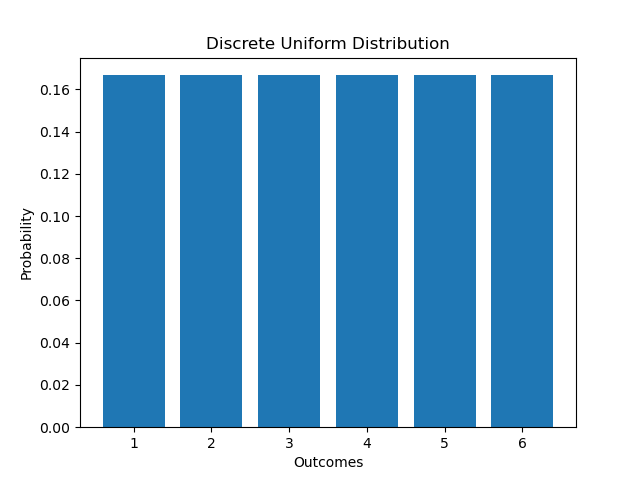
\includegraphics[width=0.8\textwidth]{./graphs/probDist/uniform_distribution.png}
\end{center}

\newpage
\subsection{Bernoulli Distribution}
The \textbf{Bernoulli Distribution} is a discrete probability distribution for a random variable that takes on only two outcomes: success (with probability \(p\)) and failure (with probability \(1 - p\)). It models the outcome of a single trial.
\[
Y \sim \text{Bern}(p)
\]
The expected value and variance are:
\[
E[Y] = p, \quad \text{Var}(Y) = p(1 - p)
\]
Key properties:
\begin{itemize}
    \item This is used to model binary outcomes (e.g., flipping a coin).
    \item The mean \(p\) is the probability of success.
\end{itemize}
\begin{center}
    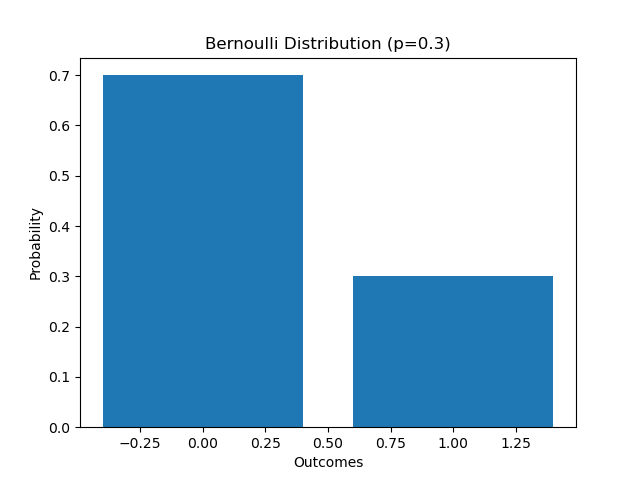
\includegraphics[width=0.8\textwidth]{./graphs/probDist/bernoulli_distribution.png}
\end{center}

\newpage
\subsection{Binomial Distribution}
The \textbf{Binomial Distribution} extends the Bernoulli distribution to multiple independent trials (e.g., flipping a coin multiple times). It models the number of successes in \(n\) trials.
\[
Y \sim B(n, p)
\]
The probability mass function (PMF) is:
\[
P(Y = y) = \binom{n}{y} p^y {(1 - p)}^{n - y}
\]
The expected value and variance are:
\[
E[Y] = np, \quad \text{Var}(Y) = np(1 - p)
\]
Key properties:
\begin{itemize}
    \item Used in scenarios where we have a fixed number of independent trials.
    \item The number of successes follows a binomial pattern.
\end{itemize}
\begin{center}
    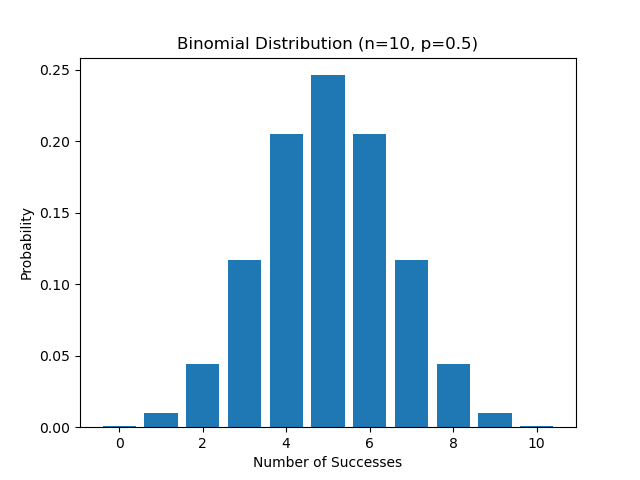
\includegraphics[width=0.8\textwidth]{./graphs/probDist/binomial_distribution.png}
\end{center}

\newpage
\subsection{Poisson Distribution}
The \textbf{Poisson Distribution} is used to model the number of occurrences of an event over a fixed interval of time or space, when these events occur with a known constant mean rate.
\[
Y \sim \text{Poisson}(\lambda)
\]
The PMF is:
\[
P(Y = y) = \frac{\lambda^y e^{-\lambda}}{y!}
\]
The expected value and variance are:
\[
E[Y] = \lambda, \quad \text{Var}(Y) = \lambda
\]
Key properties:
\begin{itemize}
    \item Useful for modeling rare events, such as the number of emails received in an hour.
\end{itemize}
\begin{center}
    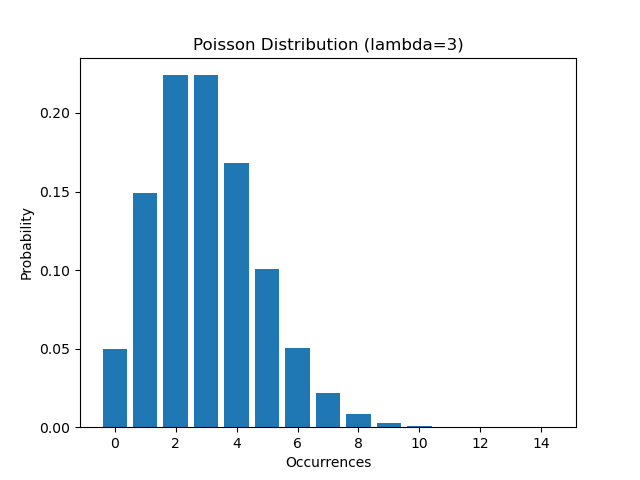
\includegraphics[width=0.8\textwidth]{./graphs/probDist/poisson_distribution.png}
\end{center}

\newpage
\section{Continuous Distributions}

\subsection{Normal Distribution}
The \textbf{Normal Distribution}, also known as the Gaussian distribution, is the most commonly encountered continuous probability distribution. Its bell-shaped curve is symmetric about the mean.
\[
Y \sim N(\mu, \sigma^2)
\]
The PDF is given by:
\[
f(y) = \frac{1}{\sqrt{2\pi\sigma^2}} e^{-\frac{{(y - \mu)}^2}{2\sigma^2}}
\]
The expected value and variance are:
\[
E[Y] = \mu, \quad \text{Var}(Y) = \sigma^2
\]
Key properties:
\begin{itemize}
    \item The Normal distribution is used in many natural phenomena (e.g., height of individuals).
    \item 68\% of values fall within one standard deviation from the mean, 95\% within two, and 99.7\% within three.
\end{itemize}
\begin{center}
    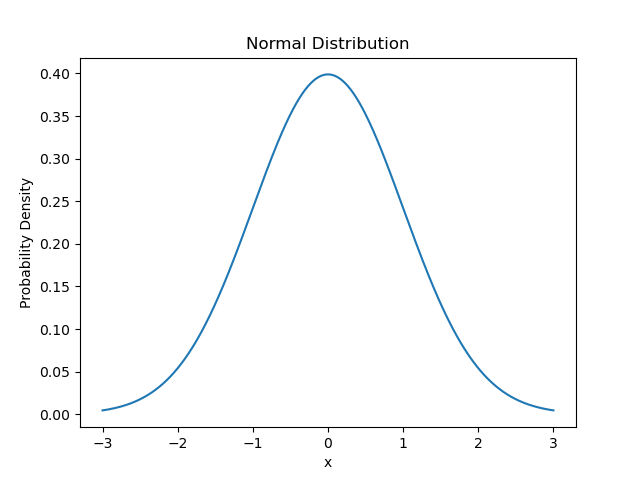
\includegraphics[width=0.8\textwidth]{./graphs/probDist/normal_distribution.png}
\end{center}

\newpage
\subsection{Student's T-Distribution}
The \textbf{Student's T-Distribution} is used when estimating the mean of a normally distributed population when the sample size is small and the population standard deviation is unknown.
\[
Y \sim t(k)
\]
The expected value and variance are:
\[
E[Y] = 0, \quad \text{Var}(Y) = \frac{k}{k-2}, \quad k > 2
\]
Key properties:
\begin{itemize}
    \item It is similar to the normal distribution but with heavier tails.
    \item Useful for confidence intervals and hypothesis testing in small samples.
\end{itemize}
\begin{center}
    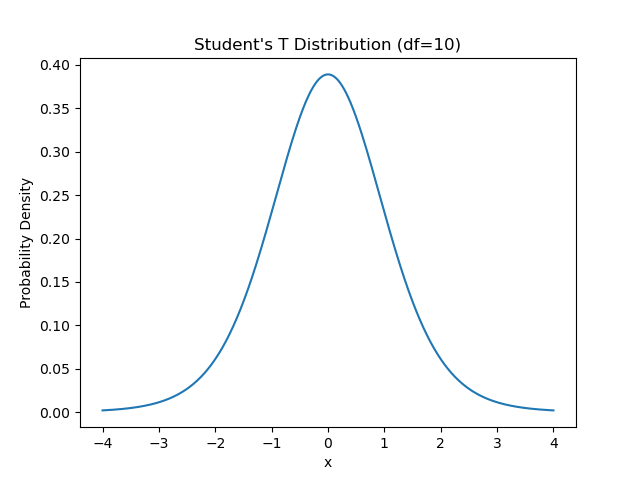
\includegraphics[width=0.8\textwidth]{./graphs/probDist/t_distribution.png}
\end{center}

\newpage
\subsection{Chi-Squared Distribution}
The \textbf{Chi-Squared Distribution} is primarily used in hypothesis testing, especially in tests of goodness of fit and tests for independence in contingency tables.
\[
Y \sim \chi^2(k)
\]
The expected value and variance are:
\[
E[Y] = k, \quad \text{Var}(Y) = 2k
\]
Key properties:
\begin{itemize}
    \item The distribution is skewed to the right, and its shape depends on the degrees of freedom \(k\).
\end{itemize}
\begin{center}
    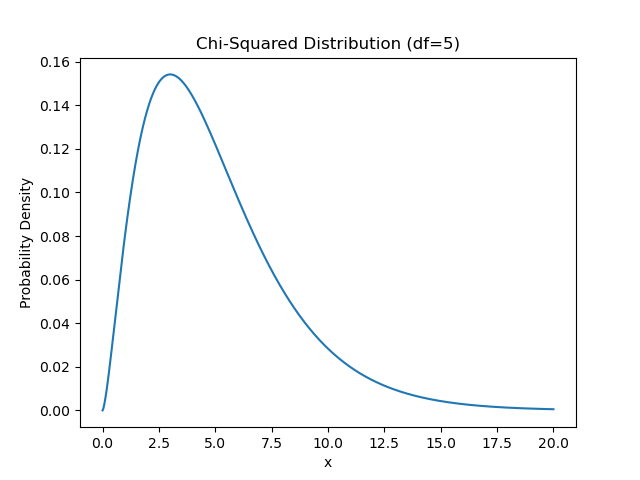
\includegraphics[width=0.8\textwidth]{./graphs/probDist/chi_squared_distribution.png}
\end{center}

\newpage
\subsection{Exponential Distribution}
The \textbf{Exponential Distribution} describes the time between events in a Poisson process, where events occur continuously and independently at a constant average rate.
\[
Y \sim \text{Exp}(\lambda)
\]
The PDF is given by:
\[
f(y) = \lambda e^{-\lambda y}, \quad y \geq 0
\]
The expected value and variance are:
\[
E[Y] = \frac{1}{\lambda}, \quad \text{Var}(Y) = \frac{1}{\lambda^2}
\]
Key properties:
\begin{itemize}
    \item Frequently used to model time-to-failure in reliability analysis.
\end{itemize}
\begin{center}
    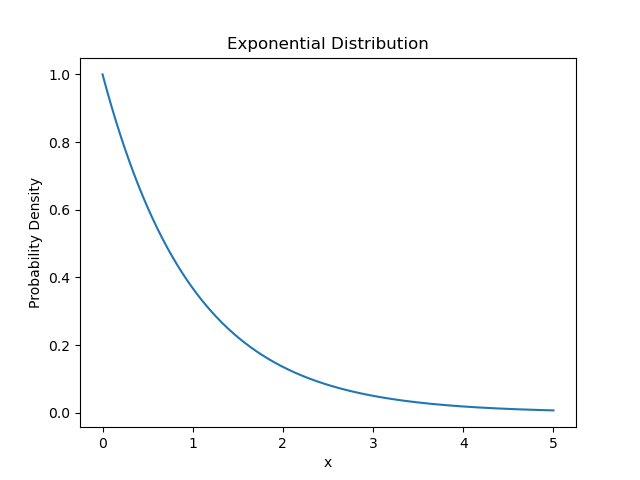
\includegraphics[width=0.8\textwidth]{./graphs/probDist/exponential_distribution.png}
\end{center}

\newpage
\subsection{Logistic Distribution}
The \textbf{Logistic Distribution} is similar to the normal distribution but has heavier tails. It is commonly used in logistic regression models.
\[
Y \sim \text{Logistic}(\mu, s)
\]
The PDF is given by:
\[
f(y) = \frac{e^{-(y-\mu)/s}}{s{(1 + e^{-(y-\mu)/s})}^2}
\]
The CDF is:
\[
F(y) = \frac{1}{1 + e^{-(y-\mu)/s}}
\]
Key properties:
\begin{itemize}
    \item It is used to model growth in social science, biology, and economics.
\end{itemize}
\begin{center}
    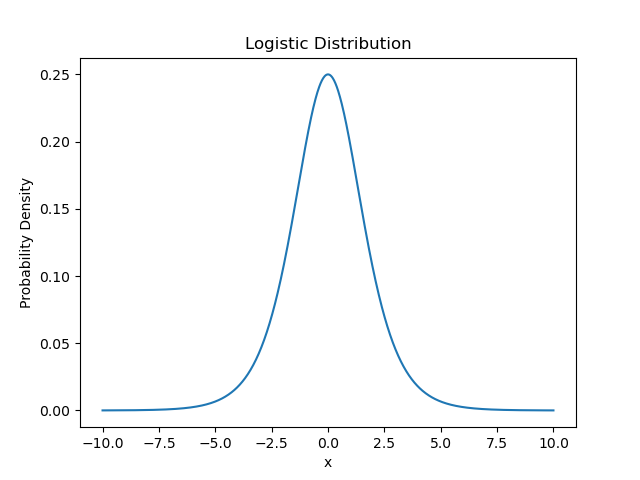
\includegraphics[width=0.8\textwidth]{./graphs/probDist/logistic_distribution.png}
\end{center}

\end{document}
